% !TEX root = ../VPJ.tex

\chapter{Visualisierung}
\label{sec:Visualisierung}

Die Auftragsplanungssoftware besitzt neben der Logik eine Visualisierung. Diese wurde mit den von Qt bereitgestellten Widgets grafisch programmiert und in der Funktion mainwindow verknüpft und organisiert. 

\section{Design}

Die Leitlinie des Grafikdesigns der HAW war:

\begin{quote}
"`Fokussiert. Direkt. Verständlich.
Und vor allem sympathisch."'	

"`Idee der neuen visuellen Sprache ist die Reduktion auf das
Wesentliche. Ziel soll es sein, einfach und klar die wichtigste
Aussage zu kommunizieren."'
\cite[4]{corporate}
\end{quote}

Beim Design der Software wurde versucht, diese Aspekte wieder aufzugreifen. Die Visualisierung sollte ebenso direkt und verständlich sein. Vor allem die Reduktion auf das Wesentliche lag besonders im Fokus. 

Um die Visualisierung im Stil der HAW zu gestalten wurde das Corporate Design bei Farb und Schriftwahl verwendet. Somit sind alle Schriftarten in der Visualisierung Open Sans. Als Farben wurden die vorgegebenen Farbstile "`HAW Hauptblau"' als Umrahmung und Abtrennung aller Bereiche gewählt. Das "`HAW Hellblau"' ist innerhalb der verschiedenen Bereiche als Trennung der Bedienelemente zu sehen. Da dieses blasser ist, können alle Bedienelemente gut erkannt und verwendet werden. 

\begin{figure}[htb]
    \centering
    
\includegraphics[width=0.3\textwidth]{Abbildungen/VPJ.png}
    \caption{VPJ-Logo}		
    \label{fig:VPJLogo}
\end{figure}

Das entworfene VPJ-Logo (Abb. \ref{fig:VPJLogo}) welches in Taskmanager, Taskleiste, an oberer Bildschirmseite und zentral in der Mitte der Visualisierung zu finden ist, unterliegt ebenfalls den Richtlinien, die im Corporate Design (vgl. \cite{corporate}) festgehalten sind. 

\section{Struktur}

Die Visualisierung lässt sich in insgesamt 6 Bereiche unterteilen. Die Bereiche sind in Abbildung \ref{fig:GesamtprogrammBereiche} dargestellt. Bereich I oben links zeigt die Fertigungsstraße mitsamt Robotern, Parkplätzen und Stationen. Dieser Bereich wird folgend Live-View genannt. 

\begin{figure}[htb]
    \centering
    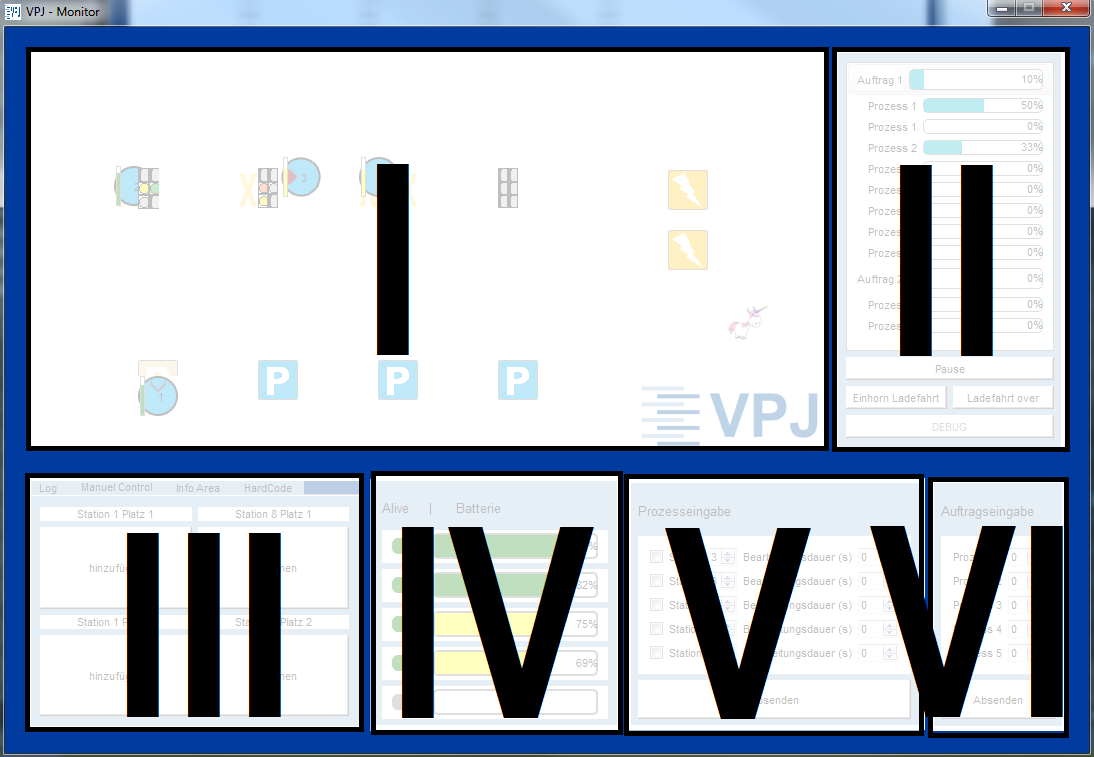
\includegraphics[width=0.8\textwidth]{Abbildungen/GesamtprogrammBereiche.png}
    \caption{Übersicht über die Bereiche innerhalb der Visualisierung}		
    \label{fig:GesamtprogrammBereiche}
\end{figure}

In Bereich II, der Auftragsübersicht, können die Fortschritte der laufenden Aufträge und Prozesse überwacht werden.

Innerhalb des Bereichs III können über Tabs vier weitere Fenster aufgerufen werden. Dabei dienen zwei der Anzeige spezifizierter Informationen, wohingegen die anderen beiden Tabs der Kontrolle dienen. Die Kombination aller vier Tabs wird folgend Tab-View genannt.

Bereich IV zeigt den Status der Robotinos an. 

Die beiden Bereiche V und VI werden ausschließlich für die Erzeugung neuer Aufträge oder Prozesse verwendet. 

In Abbildung \ref{fig:Gesamtprogramm} ist eine Übersicht der Visualisierung im laufenden Betrieb dargestellt. 

\begin{figure}[htb]
    \centering
    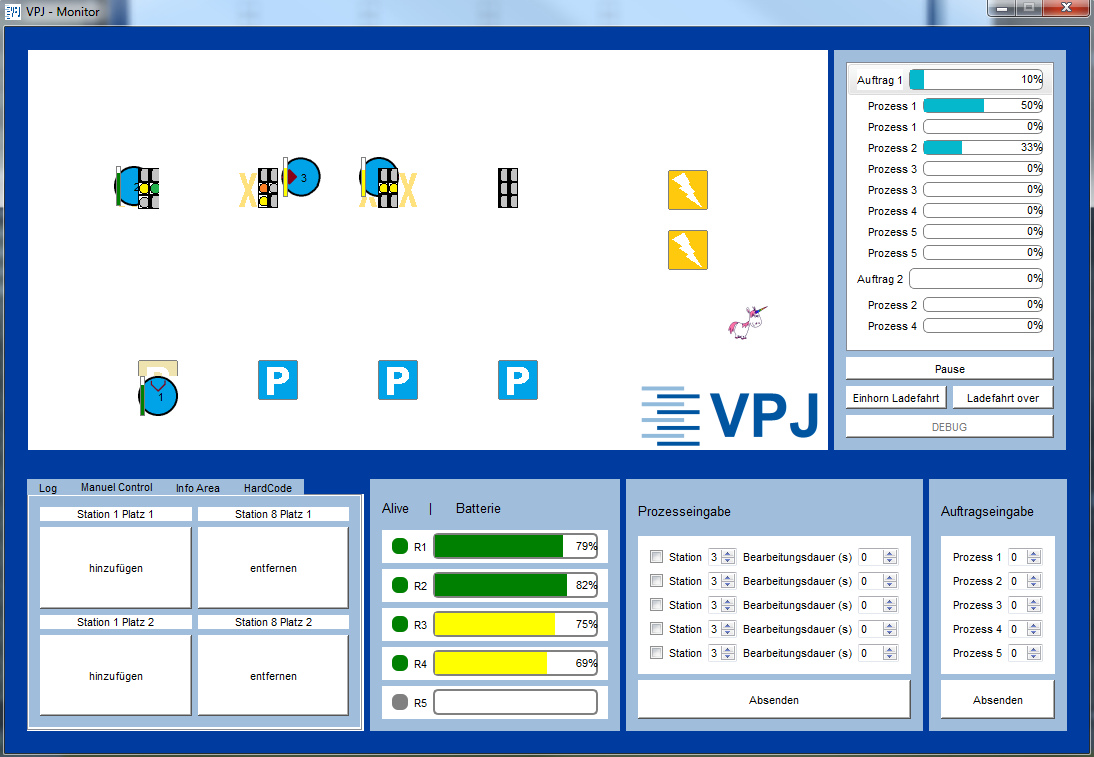
\includegraphics[width=1\textwidth]{Abbildungen/Gesamtprogramm.png}
    \caption{Übersicht Visualisierung}		
    \label{fig:Gesamtprogramm}
\end{figure}

In den folgenden Kapiteln werden die einzelnen Bereiche näher beleuchtet und ihre Implementierung in der MainWindow Funktion erläutert. 

\section{Live-View}

Der Größte der Bereiche beinhaltet eine Live-View der Fertigungsstraße, dargestellt in Abbildung \ref{fig:LiveView}. Darin sind alle Stationen, die Robotinos, Parkplätze und die Ladestationen dargestellt. In der unteren rechten Ecke ist das VPJ-Logo eingebettet. Das Fenster hat feste Maße von 800 x 400 Pixeln, wodurch die realen Raumabmessungen einfach dargestellt werden können. 1 Pixel entspricht im realen Raum 1 cm. 

\begin{figure}[htb]
    \centering
    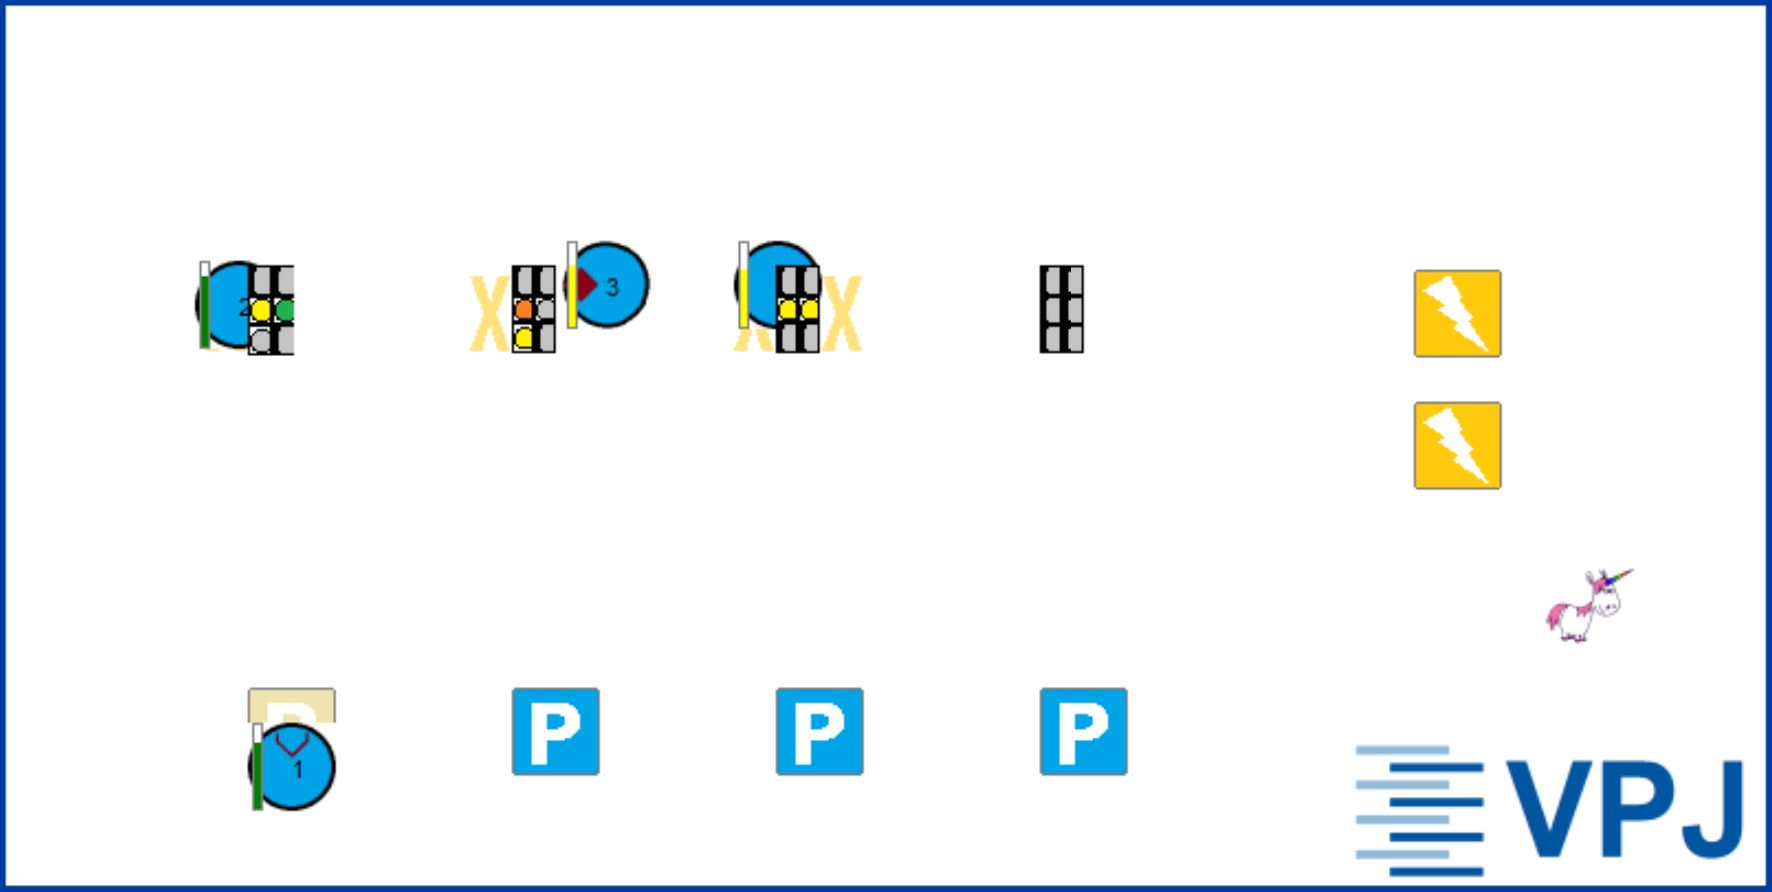
\includegraphics[width=0.9\textwidth]{Abbildungen/LiveView.png}
    \caption{Visualisierung Live-View}		
    \label{fig:LiveView}
\end{figure}

\subsection{Robotino}

Der Robotino wird immer an der Position dargestellt, die in der zugehörigen Robotinoklasse hinterlegt ist. Über die Funktion UpdateRobotinoPosition() kann eine Aktualisierung angefordert werden. Sobald der UDP-Handler neue Positionsdaten für einen Robotino empfängt und die neue Position mindestens 2 Pixel von der Alten entfernt liegt, wird diese aktualisiert. 

Die Funktion UpdateRobotinoPosition() prüft zunächst, ob der Robotino ein Hindernis erkannt hat. Bei Vorliegen eines Hindernis wird für den Robotino ein Bild geladen, welches im Rand den Hindernistyp kodiert. In Abbildung \ref{fig:RobotinoHindernis} sind alle auftretenden Hindernistypen dargestellt. Bei einem unbekannten Hindernis wird der Robotinorand Rot dargestellt, wie rechts abgebildet. Ein noch nicht klassifiziertes Hindernis wird, wie links abgebildet, mit gelbem Rand dargestellt. In der Mitte der Abbildung ist der Robotino mit orangenem Rand abgebildet, der bei einem anderen Robotino als Hindernis angezeigt wird.
Wenn kein Hindernis erkannt wird bleibt der Rand schwarz. 

\begin{figure}[htb]
    \centering
    
\includegraphics[width=0.12\textwidth]{Abbildungen/RobotinoGoffenRandGelb.png}
    
\includegraphics[width=0.12\textwidth]{Abbildungen/RobotinoGoffenRandOrange.png}
    
\includegraphics[width=0.12\textwidth]{Abbildungen/RobotinoGoffenRandRot.png}
    \caption{Robotino Darstellung bei verschiedenen Hinderniserkennungen}		
    \label{fig:RobotinoHindernis}
\end{figure}

Die Darstellung des Robotinos hängt, neben den Hindernistypen, auch von verschiedenen Stati ab. So wird ein defekter Robotino mit einer Flamme gekennzeichnet (Abb. \ref{fig:Robotino} mittig rechts). Das Einhorn als spezieller Robotino wird ebenfalls in der Darstellung als Einhorn abgebildet, in der Abbildung rechts dargestellt. 

Im Standardfall wird der Robotino wie in Abbildung \ref{fig:Robotino} links abgebildet angezeigt. Hierbei wird unterschieden ob der Greifer des Robotinos offen (links) oder geschlossen (rechts) ist. 

\begin{figure}[htb]
    \centering
    
\includegraphics[width=0.13\textwidth]{Abbildungen/RobotinoGoffen.png}
    
\includegraphics[width=0.13\textwidth]{Abbildungen/RobotinoGZu.png}
    
\includegraphics[width=0.13\textwidth]{Abbildungen/RobotinoDefect.png}
    \includegraphics[width=0.13\textwidth]{Abbildungen/Einhorn.png}
    \caption{Roboter in verschiedenen Stati (vlnr: Greifer offen, Greifer geschlossen, Defekt, Einhorn)}		
    \label{fig:Robotino}
\end{figure}

Nachdem das korrekte Bild für den Robotino ausgewählt wurde, wird dieses gleich der Ausrichtung des Robotinos gedreht. In Listing \ref{lst:RobotinoDrehung} ist die Umsetzung im Code zu sehen. Zunächst wird eine Rotationsmatrix rm in Zeile 1 erzeugt. Diese Matrix wird anhand des Winkels des Robotinos konfiguriert. Anschließend wird das Bild des Robotinos in Zeile 3 gedreht und in Zeile 4 angewendet. In Zeile 6 ist die Positionierung des gedrehten Bildes abgebildet. Da die Y-Achse des Robotino invertiert zu der Darstellung ist muss diese als Offset zu 400 angegeben werden. 

\begin{lstlisting}[frame=single, breaklines=true, numbers=left, stepnumber=2, firstnumber=1, numberstyle = \tiny, caption=Robotino Drehung ,label=lst:RobotinoDrehung]
QMatrix rm;
rm.rotate(-newPosition[2]);
QPixmap pixmap = Rlabel->pixmap()->copy().transformed(rm);
Rlabel->setPixmap(pixmap);

Robotino->move(newPosition[0]/10, 400-(newPosition[1]/10));
\end{lstlisting}

Zusätzlich zur Position beinhaltet jeder Robotino in der Mitte eine Zahl, die die eindeutige RoboterID repräsentiert. Somit kann sofort erkannt werden, welcher Robotino dargestellt ist. Außerdem ist an der linken Seite der Akkustand als vertikaler Balken dargestellt. Der Akkustand ist gleich dem, der unten im Roboterstatus-View angezeigt wird und wird dort näher beleuchtet. Am Akkustand am Robotino kann direkt erkannt werden, welcher Robotino welchen Akkustand besitzt ohne erst die IDs abgleichen zu müssen.  

\subsection{Parkplätze und Ladestationen}

Im unteren Bereich der Live-View befinden sich die vier Parkplätze für die Robotinos. Je nach Zustand werden diese verschieden dargestellt. Sobald ein Parkplatz für einen Robotino reserviert wird, oder durch einen Robotino belegt ist wird dieser in hellgelb abgebildet. 
Ein freier Parkplatz wird, wie in Abbildung \ref{fig:Parkplatz} rechts, blau dargestellt. 

Eine Aktualisierung erfolgt über den Aufruf der Funktion UpdateParkplatz() in der MainWindow. 

\begin{figure}[htb]
    \centering
    
\includegraphics[width=0.4\textwidth]{Abbildungen/Parkplatz.png}
    \caption{Visualisierung Parkplatz}		
    \label{fig:Parkplatz}
\end{figure}

Wie die Parkplätze werden auch die Ladestationen entweder reserviert (Abb. \ref{fig:Ladestation} oben) in blassem hellgelb dargestellt, oder in kräftigem Gelb für freie Ladestationen (Abb. \ref{fig:Ladestation} unten). 

\begin{figure}[htb]
    \centering
    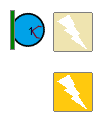
\includegraphics[width=0.25\textwidth]{Abbildungen/Laden.png}
    \caption{Visualisierung Ladestation}		
    \label{fig:Ladestation}
\end{figure}

\subsection{Stationen}

Die Stationen enthalten Informationen über die Werkstücke, die an ihnen bearbeitet werden. Es gibt insgesamt 8 Stationen, wobei immer zwei Stationen horizontal zusammengefasst sind. Ein solcher Stationsverbund ist in Abbildung \ref{fig:Station} abgebildet. Der oberste Kreis einer Station repräsentiert den RFID-Kopf. Darunter befinden sich die beiden Arbeitsplätze. Jeder Arbeitsplatz enthält in seiner Farbkodierung eine Information über das Werkstück. In der Abbildung sind alle möglichen Farbkodierungen dargestellt.

\begin{figure}[htb]
    \centering
    
\includegraphics[width=0.18\textwidth]{Abbildungen/Station.png}
    \caption{Stationen mit verschiedenen Arbeitsplatzstati}		
    \label{fig:Station}
\end{figure}

Sobald ein Arbeitsplatz reserviert wird, da sich ein Werkstück auf dem Weg dahin befindet, ist dieser Gelb dargestellt. Ein roter Arbeitsplatz zeigt an, das dieser defekt ist und nicht mehr angefahren werden kann. Ein defekter Arbeitsplatz wird von der Auftragsplanung nicht mehr berücksichtigt. Diese Einstellung kann mit der Hard-Code Area erzeugt werden. Wenn ein Werkstück an den Arbeitsplatz abgelegt wird befindet sich dieses in Bearbeitung und der Platz wird Orange dargestellt. Sobald die Bearbeitung abgeschlossen ist, wechselt die Farbe des Arbeitsplatz auf Grün und das Werkstück ist bereit zur Abholung. Ein leerer Arbeitsplatz wird in neutralem grau dargestellt. 

Über die Funktion UpdateStationsplatz() kann die Farbkodierung eines einzelnen Arbeitsplatz anhand des übergebenen Status angepasst werden. 

Zusätzlich zu den Arbeitsplatzstati wird neben jeder Station angezeigt, ob diese reserviert ist. Da nicht zwei Robotinos gleichzeitig zu einer Station fahren sollen, werden diese, sobald sich ein Robotino auf dem Weg dahin befindet oder an einer Station arbeitet, reserviert. Eine reservierte Station ist in der Visualisierung an dem hellgelben X neben der Station zu erkennen. In Abbildung \ref{fig:Station} ist die linke Station reserviert und die rechte Station frei. Mit der Funktion UpdateStation() kann die Reservierung für eine Station angepasst werden. 

Im Normalbetrieb, ohne die Zusatzfunktionalität der Hard-Code Area, bewirkt ein Klick auf einen Arbeitsplatz eine Aktualisierung der Timestamp-Area. 

\section{Auftragsübersicht}
\label{sec:Auftragsuebersicht}

Der rechte Bereich (II) in der Visualisierung enthält die Auftragsübersicht. In Abbildung \ref{fig:Auftragsfortschritt} ist zu erkennen, dass sich der Bereich in zwei Teile aufteilt. Der obere Teil ist für die Anzeige der Aufträge und Prozesse zuständig. Im unteren Teil kann über bereitgestellte Buttons interagiert werden.

\begin{figure}[htb]
    \centering
    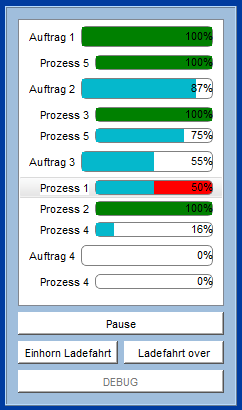
\includegraphics[width=0.4\textwidth]{Abbildungen/Auftragsfortschritt.png}
    \caption{Auftragsfortschritt}		
    \label{fig:Auftragsfortschritt}
\end{figure}

\subsection{Auftragsdarstellung}

In der Abbildung \ref{fig:Auftragsfortschritt} ist zu erkennen, dass jeder Auftrag dargestellt wird, inklusive seiner enthaltenen Prozesse. Durch Anklicken eines Auftrags der Liste können die zugehörigen Prozesse eingeblendet (Abb. \ref{fig:Auftragsausblendung} links) oder ausgeblendet (Abb. \ref{fig:Auftragsausblendung} rechts) werden. 

\begin{figure}[htb]
    \centering
    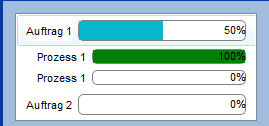
\includegraphics[width=0.4\textwidth]{Abbildungen/AuftragAusgeklappt.png}
    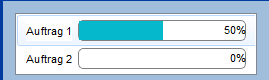
\includegraphics[width=0.4\textwidth]{Abbildungen/AuftragEingeklappt.png}
    \caption{Auftrag ein- und ausgeblendet}		
    \label{fig:Auftragsausblendung}
\end{figure}

Der im Auftrag (siehe Kapitel \ref{sec:Auftrag}) und Prozess (siehe Kapitel \ref{sec:Prozess}) gespeicherte Fortschritt wird im Fortschrittsbalken aktualisiert, wenn die Funktion UpdateAuftragsFortschritt() innerhalb des Auftragsitem aufgerufen wird. Sobald der Fortschritt 100 Prozent erreicht, wird der Balken grün gefärbt. Der Balken eines geblockten Prozesses wird rot eingefärbt(siehe Abb. \ref{fig:Auftragsfortschritt} Auftrag 3 Prozess 1). 

\subsubsection{Auftragsitem}

Das Auftragsitem (siehe Kapitel \ref{sec:Auftragsitem}) wird in der Auftragsübersicht mit einem Textfeld und nebenstehendem Fortschrittsbalken visualisiert (Abb. \ref{fig:Auftragsitem} links). Das Textfeld enthält dabei die Auftragsnummer. Das gesamte Auftragsitem hat eine Höhe von 31 Pixeln, die Breite ist variabel. 

\begin{figure}[htb]
    \centering
    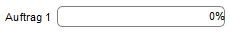
\includegraphics[width=0.4\textwidth]{Abbildungen/Auftragsitem.png}
    
\includegraphics[width=0.4\textwidth]{Abbildungen/Prozessitem.png}
    \caption{Auftragsitem (links) und Prozessitem (rechts)}		
    \label{fig:Auftragsitem}
\end{figure}

Sowohl Auftrags als auch Prozessitem sind als QListWidgetItem (siehe Kapitel \ref{sec:QListWidgetItem}) implementiert.

Wenn ein QListWidgetItem angeklickt wurde, wird die Funktion on\_Auftrags\-List\-Widget\-\_item\-Clicked() aufgerufen. In Listing \ref{lst:AuftragsitemClicked} ist der Code dargestellt, der dabei für ein Auftragsitem ausgeführt wird. Zunächst wird geprüft, ob das angeklickte Item ein Prozessitem oder ein Auftragsitem ist (Zeile 1). Wenn es sich um ein Auftragsitem handelt, wird die Zeile des angeklickten Items zwischengespeichert (Zeile 3). Anschließend wird für jedes nachfolgende Item geprüft, ob es existiert und ein Prozessitem ist. Solange dabei weitere Prozessitems gefunden werden, werden diese ein- oder ausgeblendet, abhängig davon ob diese zuvor ein- oder ausgeblendet waren. Ansonsten wird die Funktion verlassen.

\begin{lstlisting}[frame=single, breaklines=true, numbers=left, stepnumber=2, firstnumber=1, numberstyle = \tiny, caption=Funktionsblock nach Klicken auf Auftragsitem ,label=lst:AuftragsitemClicked]
if ((item->whatsThis() == WhatsThis[0]))
{
    int itemrow = AuftragListWidget->row(item);
    while (true)
    {
        QListWidgetItem* tempitem = AuftragListWidget->item(itemrow+1);
        if (tempitem == nullptr || (tempitem->whatsThis() == WhatsThis[0]))
        {
            break;
        }
        tempitem->setHidden(!tempitem->isHidden());
        itemrow++;
        continue;
    }
}
\end{lstlisting}

Dadurch können durch Anklicken eines Auftragsitem die zugehörigen Prozessitems angezeigt oder ausgeblendet werden. Prozesse eines anderen Auftrags werden dabei ignoriert.

\subsubsection{Prozessitem}

Das Prozessitem (Abb. \ref{fig:Auftragsitem} rechts) wird in der Auftragsübersicht ähnlich dem Auftragsitem dargestellt. Der Hauptunterschied ist hierbei, dass das Prozessitem eine Höhe von nur 21 Pixeln besitzt und weiter eingerückt wird, als ein Auftragsitem. Dadurch kann die Hierarchie zwischen Aufträgen und Prozessen einfach erkannt werden. 

Wenn nach Anklicken eines QListWidgetItems dieses in der Funktion on\_\-Auftrags\-List\-Widget\_\-item\-Clicked() als Prozessitem identifiziert wurde, wird der in Listing \ref{lst:ProzessitemClicked} dargestellte Code ausgeführt. 

\begin{lstlisting}[frame=single, breaklines=true, numbers=left, stepnumber=2, firstnumber=1, numberstyle = \tiny, caption=Funktionsblock nach Klicken auf Prozessitem ,label=lst:ProzessitemClicked]
else if (item->whatsThis() == WhatsThis[1])
{
    Prozessitem *pi = dynamic_cast<Prozessitem*>(AuftragListWidget->itemWidget(item));
    QPushButton *p = GetPressedHardCodeButton();
    if (p == ButtonBlockAuftrag)
    {
        pi->prozess->SetBlocked();
        pi->UpdateProzessBlocked();
    }
}
\end{lstlisting}

Dabei wird das QListWidgetItem zunächst dynamisch in Zeile 3 auf ein Prozessitem gecasted. 

In C++ gibt es verschiedene Wege ein Objekt in ein anderes zu casten. Die geläufigsten (regulären) Castvorgänge sind reinterpret\_cast oder const\_cast. Neben diesen gibt es Funktionen wie dynamic\_cast oder static\_cast. Ein regulärer Cast versucht, aus allen weiteren möglichen regulären Castvarianten eine geeignete zu finden, die funktioniert. Dynamic\_cast, oder static\_cast wird hierbei nicht berücksichtigt. Der Unterschied zwischen static\_cast und dynamic\_cast ist hauptsächlich, dass für einen static\_cast bekannt sein muss, in was das Objekt gecastet werden soll. Ein dynamic\_cast hingegen kann immer ausgeführt werden und liefert einen Nullpointer zurück, wenn der Cast fehlschlägt. In diesem Fall wurde die weniger verbreitete Funktion dynamic\_cast gewählt, da nur diese alle Anforderungen zur Laufzeit unterstützt (vgl. \cite{cast}). 

Der Cast ist notwendig, da das allgemeine QListWidgetItem nicht auf die Funktionen zugreifen kann, die das Prozessitem zur Verfügung stellt. 

Nachdem sichergestellt wurde, dass das Objekt ein Prozessitem ist, wird in Zeile 4 ausgewertet, ob der Hard-Code Button zum blockieren eines Prozesses aktiv ist und anschließend dieser Prozess dahingehend aktualisiert.

Bei einem Doppelklick auf ein QListWidgetItem wird die Funktion on\_Auf\-trags\-List\-Widget\_item\-Double\-Clicked() aufgerufen (siehe Listing \ref{lst:ProzessitemDoubleClicked}). Hierin wird überprüft, ob das angeklickte Objekt ein Prozessitem war und dieses gegebenenfalls gecastet. Auf dem gecasteten Objekt kann dann ein Signal emittiert werden, das eine Aktualisierung der Timestamps bewirkt. 

\begin{lstlisting}[frame=single, breaklines=true, numbers=left, stepnumber=2, firstnumber=1, numberstyle = \tiny, caption=Funktionsblock nach Doppelklick auf Prozessitem ,label=lst:ProzessitemDoubleClicked]
Prozessitem *pi = dynamic_cast<Prozessitem*>(AuftragListWidget->itemWidget(item));
emit GetTimestampsOnProzessClicked(pi->prozess->lfdId);
\end{lstlisting}

\subsection{Buttons der Auftragsübersicht}

Um die im Einhorn (Robotino 5) fest einprogrammierte Ladefahrt zu starten, wurden die Buttons "`Einhorn Ladefahrt"' und "`Ladefahrt over"' implementiert. Jede Betätigung des Buttons  "`Einhorn Ladefahrt"' bewirkt ein einmaliges Senden eines definierten Auftrags an Robotino 5 (siehe Kapitel \ref{sec:Telegramme}). Dazu wird die Funktion EinhornLaden() im UDP-Handler genutzt. 
 
Über eine Betätigung des Buttons "`Pause"' wird die Auftragsvergabe in der State-Machine der Fertigungsplanung pausiert. Somit werden Keine Transportaufträge mehr an die Robotinos versendet. Ladefahrten oder eine Parkplatzfahrt werden weiterhin zugelassen. Der Pause Button wird getoggelt, das heißt wenn er betätigt wird, bleibt er bis zur erneuten Betätigung aktiv. Um zu erkennen, dass die Auftragsplanung pausiert ist, wird der Button im aktivierten Zustand, wie in Abbildung \ref{fig:Pause} zu sehen, Rot hervorgehoben.

\begin{figure}[htb]
    \centering
    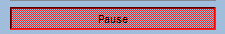
\includegraphics[width=0.4\textwidth]{Abbildungen/Pause.png}
    \caption{Pause Button gedrückt}		
    \label{fig:Pause}
\end{figure}

Die Auftragsplanung wird beispielsweise pausiert, wenn ein Robotino ausgefallen ist und über die Hard-Code Area die Fertigungsstraße wieder aufgeräumt werden muss. 

\section{Tab-View}

Der Bereich III unten links wurde als Tab-View umgesetzt. Es kann jederzeit einer aus vier verschiedenen Tabs ausgewählt werden, welcher angezeigt wird. Zwei der Tabs dienen der Anzeige, über die anderen beiden kann das Programm bedient werden. 

Auf die einzelnen Tabs wird in den folgenden Abschnitten genauer eingegangen. 

\subsection{Log-View}

Der erste Tab, der auch bei Programmstart geöffnet ist, beinhaltet das Log (Abbildung \ref{fig:Log}). In diesem Tab ist keine Eingabe möglich. Im scrollbaren Textfenster werden zu Programmlaufzeit Logeinträge dargestellt, die durch den Programmablauf generiert wurden. 

\begin{figure}[htb]
    \centering
    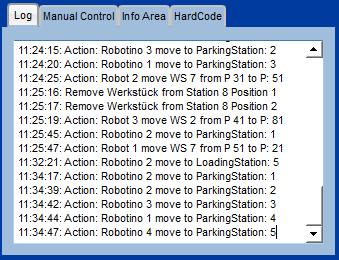
\includegraphics[width=0.6\textwidth]{Abbildungen/Log.png}
    \caption{Tab: Log View}		
    \label{fig:Log}
\end{figure}

Über die Funktion WriteToDebugTextArea() kann ein übergebener String an das Textview angehängt werden. So wird im Textfeld eine neue Zeile hinzugefügt. Dem übergebenen String wird zuvor der aktuelle Zeitstempel vorangestellt. 

Eine Liste der vorkommenden Logeinträge ist in Tabelle \ref{tab:Log} zu finden. 

\begin{table}[!ht]
	\centering
	\begin{tabular}{|c|c|p{10cm}|}
		\hline
		Nr & Kategorie &	Nachricht \\
		\hline
    1  & Initialisierung & Fertigungsplanung initialisiert \\
    2  & Initialisierung & Datenbank gestartet \\
    3  & Initialisierung & Fertigungsplanung gestartet \\
 		\hline
    4  & Feedback & Prozess hinzugefügt \\
    5  & Feedback & Auftrag hinzugefügt \\
    6  & Feedback & Add Werkstück to Station 1 Position 1 \\
    7  & Feedback & Remove Werkstück from Station 8 Position 1 \\
 		\hline
    8  & Aktion & Action: Robotino 1 move to LoadingStation: 5 \\
    9  & Aktion & Action: Robotino 1 move to ParkingStation: 1 \\
    10 & Aktion & Action: Robotino 1 move WS 2 from Position 11 to Position 22 \\
 		\hline
    11 & Warnung & Warning: Robot 1 died \\
    12 & Warnung & Warning: Robotino 1 exploded \\
    13 & Info & Info: Robotino 1 repaired \\
		\hline
    14 & Error & ERROR: Could not set Station Place ready after Prozess Timer elapsed \\
    15 & Error & ERROR: Could not set Station Place full after Greifer opened \\
    16 & Error & ERROR: Could not set Source Station Place free after Robot Greifer closed \\
    17 & Error & ERROR: Could not set Loading Station Place free after Robot drove away \\
    18 & Error & ERROR: Robot not found \\
    19 & Error & ERROR: Could not set Station place free from Hard Code Button \\
    20 & Error & ERROR: Could not set Station place defect from Hard Code Button \\
    21 & Error & ERROR: Could not set Station free from Hard Code Button \\
    22 & Error & ERROR: Could not set Loading Station Place reserved after sending Task to Robot \\
    23 & Error & ERROR: Could not set Parking Station Place reserved after sending Task to Robot \\
    24 & Error & ERROR: Could not set Target Station Place reserved after sending Task to Robot \\
    25 & Error & ERROR: Could not set Source Station Place reserved after sending Task to Robot \\
		\hline
    26 & Roboter Error & ROBOTERROR: Robot 1 lost Werkstueck \\
    27 & Roboter Error & ROBOTERROR: Robot 1 was not able to grab Werkstueck \\
    28 & Roboter Error & ROBOTERROR: Robot 1 was not able to plan Route \\
		\hline
	\end{tabular}
	\caption{Logeinträge}
	\label{tab:Log}
\end{table}

Aus der Tabelle kann weiterhin entnommen werden, dass die einzelnen Logeinträge in Kategorien eingeteilt werden können. Die Kategorie Initialisierung zeigt an, dass das Programm erfolgreich gestartet wurde und bereit ist für Eingaben vom Benutzer. 

Die Logeinträge der Kategorie Feedback zeigen dem Benutzer, dass eine von ihm getätigte Eingabe erfolgreich interpretiert und ausgeführt wurde. Dazu zählt das Hinzufügen oder Entfernen von Werkstücken an die Stationen oder das Hinzufügen von Prozessen oder Aufträgen. 

Die Aktionen beschreiben die von den Robotinos ausgeführten Tätigkeiten und werden immer bei erfolgreicher Auftragsvergabe an einen Robotino dem Log hinzugefügt. 

Um eine Warnung zu erzeugen, muss ein Roboter entweder die Kommunikation verloren haben, oder aktiv auf defekt geschaltet worden sein. 

Auf einen Error muss individuell reagiert werden. Während des regulären Betriebs sollte keiner der Errors auftreten. Ein Error zeigt somit eine Fehlfunktion des Programms an, und weist auf den Moment des Auftretens hin.

Die Roboter-Error werden vom Robotino gesendet. Auf diese muss der Anwender händisch reagieren. Die einzelnen Errortypen und die nötige Reaktion sind in Kapitel \ref{sec:Error} beschrieben. 

Während des normalen Betriebs besteht das Log zum größten Teil aus Einträgen der Kategorie Aktion, ergänzt um einzelne Feedback-Einträge (siehe Snapshot in Abb. \ref{fig:Log}).  

\subsection{Manual Control}

Der zweite Tab der Tab-View, Abbildung \ref{fig:ManualControl}, enthält Buttons zum manuellen Hinzufügen und Entfernen von Werkstücken. 

\begin{figure}[htb]
    \centering
    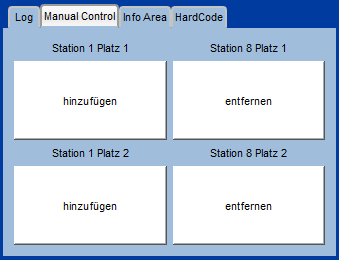
\includegraphics[width=0.6\textwidth]{Abbildungen/ManualControl.png}
    \caption{Tab: Manual Control}		
    \label{fig:ManualControl}
\end{figure}

Über die beiden linken Buttons können dem Rohteillager einzelne Werkstücke zugeteilt werden. Dazu muss zuvor ein Werkstück händisch der realen Fertigungsstraße an entsprechender Position eingelegt werden. 

Um die fertig bearbeiteten Teile aus Station 8 zu entfernen, können die beiden rechten Buttons verwendet werden. 

Über einen Action-Listener wird beim Klick auf einen der Buttons eine zugeordnete Funktion, z.B. on\_S1P2add\_clicked(), aufgerufen. In der aufgerufenen Funktion wird ein Signal emittiert, dass in der Fertigungsplanung ein Werkstück an entsprechender Stelle der Fertigungsstraße hinzufügt oder entfernt. 

\subsection{Timestamp-Area}

Im dritten Tab der Tab-View erfolgt eine Anzeige der in der Datenbank gespeicherten Timestamps. Es gibt zwei Arten, Timestamps anzeigen zu lassen. Diese sind in Abbildung \ref{fig:InfoArea} dargestellt. 

\begin{figure}[htb]
    \centering
    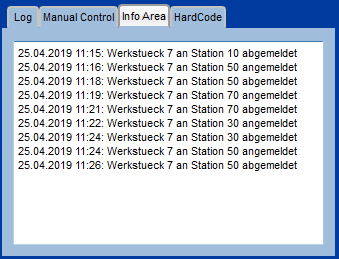
\includegraphics[width=0.4\textwidth]{Abbildungen/TimestampsWerkstueck.png}
    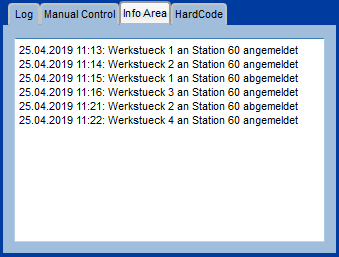
\includegraphics[width=0.4\textwidth]{Abbildungen/TimestampsStation.png}
    \caption{Tab: Info Area}		
    \label{fig:InfoArea}
\end{figure}

Es können entweder alle Timestamps eines bestimmten Werkstücks (Abb. \ref{fig:InfoArea} links) oder alle Timestamps einer Station (Abb. \ref{fig:InfoArea} rechts) angezeigt werden.

Im Timestamp ist beschrieben, zu welcher Zeit sich ein Werkstück an welcher Station an-, bzw. abgemeldet hat. Man kann feststellen, dass sich an Station 1 nur Werkstücke abmelden und an Station 8 nur Werkstücke anmelden, da diese hier jeweils händisch ergänzt bzw. entnommen werden. 

Um die Timestamps einer Station anzuzeigen, muss ein leerer Arbeitsplatz oder der RFID-Platz angeklickt werden. Dadurch wird die Funktion SetTimestamps() aufgerufen, welche das Textview aktualisiert. 

Timestamps für ein spezielles Werkstück können angezeigt werden, indem ein dem Werkstück zugeordneter Arbeitsplatz angeklickt wird. Dabei ist es egal, ob sich das Werkstück gerade auf diesem befindet, oder nur eine Reservierung vorliegt. Alternativ kann, um auch abgeschlossene Werkstücke darstellen zu können, auf das zugehörige Prozessitem in der Auftragsübersicht ein Doppelklick gemacht werden. Dadurch werden die zugehörigen Timestamps dargestellt. 

\subsection{Hard-Code Bereich}
\label{sec:HardCode}

Der Hard-Code Tab wird benötigt, um die Programmlogik gezielt zu umgehen, oder Stati "`hart"' zu überschreiben oder zu setzen. Dazu wurden die in Abbildung \ref{fig:HardCode} dargestellten Buttons implementiert. Jeder Button hat eine eigene Funktion und wird in den folgenden Abschnitten einzeln beleuchtet. 

\begin{figure}[htb]
    \centering
    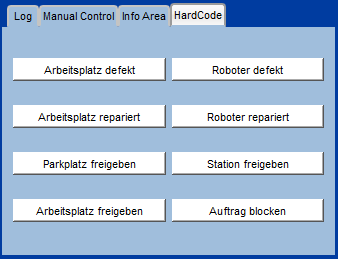
\includegraphics[width=0.6\textwidth]{Abbildungen/HardCode.png}
    \caption{Tab: Hard-Code}		
    \label{fig:HardCode}
\end{figure}

Die Betätigung eines Buttons versetzt die Visualisierung in den "`Hard-Code Modus"'. Der betätigte Button bleibt dabei gedrückt und indiziert, welche Funktionalität aktiv ist. Um nicht versehentlich im Hard-Code Modus Dinge zu überschreiben wird das Live-View rot eingefärbt. Ein Vergleich der normalen Visualisierung und des Hard-Code Modus ist in Abbildung \ref{fig:GesamtprogrammROT} dargestellt. Es ist gut zu erkennen, dass der Hard-Code Modus nicht übersehen werden kann. 

\begin{figure}[htb]
    \centering
    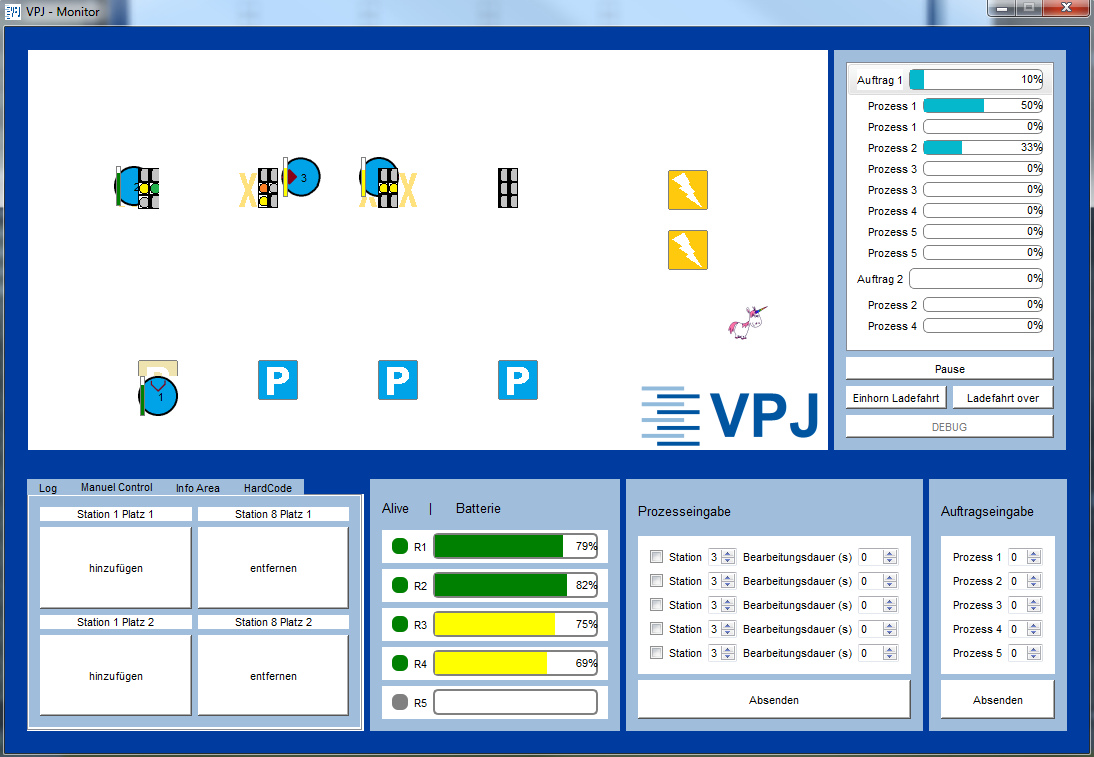
\includegraphics[width=0.45\textwidth]{Abbildungen/Gesamtprogramm.png}
    \includegraphics[width=0.45\textwidth]{Abbildungen/GesamtprogrammROT.png}
    \caption{Vergleich Visualisierung - Normal VS Hard-Code Modus}		
    \label{fig:GesamtprogrammROT}
\end{figure}

Der Hard-Code Modus kann durch Betätigen des aktiven Buttons wieder verlassen werden. 

Um sicherzustellen, dass zeitgleich immer nur eine Hard-Code Funktionalität aktiv ist, wird bei Pressen eines Buttons, nach der Button-Listenerfunktion, zuerst die Funktion ResetButtonsExceptOne() aufgerufen, wenn der Button noch nicht aktiv war. In dieser Funktion wird der Hintergrund der Live-View rot eingefärbt. Anschließend werden alle Buttons die sich, neben dem Angeklickten, im Hard-Code Tab befinden deaktiviert. 

Die Funktion GetPressedHardCodeButton() liefert für den Fall, dass ein Button aktiviert ist, diesen als Rückgabewert zurück. 

\subsubsection{Arbeitsplatz im Hard-Code}

Wenn der Button "`Arbeitsplatz defekt"' aktiviert, und ein Arbeitsplatz angeklickt wird, so wird der Status dieses Arbeitsplatzes in der Fertigungsstraße zu defekt gesetzt. Die Visualisierung wird dadurch ebenfalls aktualisiert. 

Gegenteilig dazu kann, über den Button "`Arbeitsplatz repariert"', ein zuvor defekt geschalteter Arbeitsplatz durch Anklicken wieder freigegeben werden. 

Um bei Anklicken des Arbeitsplatzes nicht nur den Timestamp auszugeben, wird in der Funktion StationClicked() zunächst über den Rückgabewert der Funktion GetPressedHardCodeButton() ausgewertet, ob einer der beschriebenen Buttons nicht aktiviert ist. 

\subsubsection{Robotino im Hard-Code}

Ähnlich dem Arbeitsplatz kann über den Button "`Roboter defekt"' der Status des angeklickten Robotinos auf defekt gesetzt werden. Dieser wird dadurch von der Auftragsplanung ausgeschlossen und bekommt als Visualisierung die Flamme. 

Ein Robotino muss defekt geschaltet werden, wenn sich dieser aufgehängt hat, die Kommunikation zum Robotino fehlschlägt oder andere Probleme an dem Robotino auftreten. Ein Entfernen eines nicht defekt geschalteten Robotinos kann zu einer Auftragsvergabe an den nicht vorhandenen Roboter führen. Durch die implementierten Timeouts würde das Programm zwar weiterlaufen, allerdings in deutlich verlangsamter Form, sobald es dem defekten Robotino einen Auftrag erteilen möchte. 

Der Button "`Roboter repariert"' aktiviert den angeklickten (defekten) Robotino wieder. 

Die dazu verwendete Funktion heißt RobotClicked().

\subsubsection{Freigabefunktionen}

Nach einem Ausfall eines Robotinos, während dieser bereits einen Auftrag erhalten hatte, müssen eventuelle Reservierungen gelöscht werden. Dafür sind die Buttons "`Parkplatz freigeben"', "`Arbeitsplatz freigeben"', und "`Station freigeben"' vorgesehen.

Der Button "`Station freigeben"' bewirkt, dass die angeklickte Station nicht mehr von einem Robotino blockiert wird. Dazu wird in Datenbank und Fertigungsplanung der Stationsstatus als frei markiert. Um eine Station freizugeben kann ein beliebiger zur Station gehöriger Arbeitsplatz angeklickt werden.

Ebenso wird mit Parkplätzen und Ladestationen verfahren. Da sich diese in der Implementierung nicht unterscheiden, werden beide über den Button "`Parkplatz freigeben"' wieder auf frei gesetzt. 

Mit dem Button "`Arbeitsplatz freigeben"' können reservierte oder belegte Arbeitsplätze durch Anklicken zu freien Arbeitsplätzen zurückgesetzt werden. 

\subsubsection{Auftrag blocken}

Über den Button "`Auftrag blocken"' kann ein Prozess eines Auftrags abgebrochen werden. Dazu muss im Hard-Code Modus der abzubrechende Prozess in der Auftragsübersicht angeklickt werden. Dieser wird dann rot markiert und intern als geblockt behandelt. 

Ein Auftrag muss geblockt werden, wenn während des Ablaufs ein unvorhergesehenes Ereignis die weitere Bearbeitung des Auftrags verhindert. Dazu zählt beispielsweise ein Totalausfall des bearbeitenden Robotinos, Verlust des Werkstücks oder anderweitig fehlgeschlagener Transport. 

Wenn ein Auftrag geblockt wurde, sollte das zugehörige Werkstück aus der Fertigungsstraße entfernt werden. 

\section{Roboterstatus}

In Bereich IV wird der Status jedes Robotinos dargestellt. Dabei ist auf der linken Seite der Alive-Status der Robotinos, und auf der rechten Seite der Akkustand dargestellt (Abb. \ref{fig:Batterie}). 

\begin{figure}[htb]
    \centering
    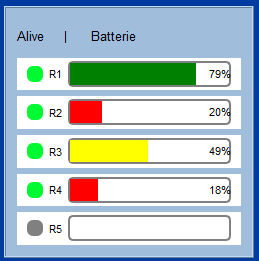
\includegraphics[width=0.5\textwidth]{Abbildungen/Batterie.png}
    \caption{Batterie und Statusanzeige}		
    \label{fig:Batterie}
\end{figure}

\subsection{Akkustand}

Innerhalb der MainWindow wird die Funktion UpdateRobotinoAkku genutzt, um den Akkustand zu aktualisieren. Dabei wird unterschieden, wie hoch der Akkustand ist. Bei einem Akkustand von kleiner als 30 Prozent wird der Fortschrittsbalken rot eingefärbt (Abb. \ref{fig:Batterie} R2, R4). Der Robotino wird bei <25 Prozent Akku zur Ladestation geschickt. 

Ein Akkustand von über 77 Prozent wird, wie in Abbildung \ref{fig:Batterie} R1, grün dargestellt. Bei einem Akkustand zwischen 30 und 77 Prozent wird der Fortschrittsbalken gelb dargestellt (Abb. \ref{fig:Batterie} R3). 

Die Anpassung der Farbe geschieht über das Setzen des Stylesheet für den Fortschrittsbalken. In Listing \ref{lst:ProgressbarStylesheet} ist das implementierte Stylesheet für alle Fortschrittsbalken dargestellt. 

\begin{lstlisting}[frame=single, breaklines=true, numbers=left, stepnumber=2, firstnumber=1, numberstyle = \tiny, caption=Progressbar Stylesheet ,label=lst:ProgressbarStylesheet]
QProgressBar {
    border: 2px solid grey;
    border-radius: 5px;
	text-align: right;
 }

 QProgressBar::chunk {
     background-color: #05B8CC;
     width: 2px;
 }

font: 8pt "OpenSans";
background-color: rgb(160 ,190, 220);
\end{lstlisting}

Indem der in Listing \ref{lst:AkkuStylesheet} dargestellte Code in der UpdateRobotinoAkku() Funktion ausgeführt wird, wird die Farbe des jeweiligen Fortschrittsbalken-Chunk überschrieben und somit angepasst. In Zeile 1 erfolgt die Aktualisierung des Fortschrittsbalken in der Roboterstatus-View. Zeile 2 zeigt die anschließende Aktualisierung des vertikalen Fortschrittsbalken am Robotino. 

\begin{lstlisting}[frame=single, breaklines=true, numbers=left, stepnumber=2, firstnumber=1, numberstyle = \tiny, caption=Stylesheet Aktualisierung der Akku-Progressbar ,label=lst:AkkuStylesheet]
P->setStyleSheet("QProgressBar::chunk {background-color: green}");
Pklein->setStyleSheet("QProgressBar::chunk {background-color: green}");
\end{lstlisting}

\subsection{Alive-Status}

Der linke Bereich des Roboterstatus-View enthält die Information zum Alive-Status des Robotinos (vgl. \ref{sec:Robotino}). Die dargestellte grüne LED blinkt, während der Roboter als "`lebend"' gilt. Das Blinken ist in Abbildung \ref{fig:Led} abgebildet. 

\begin{figure}[htb]
    \centering
    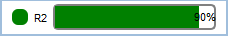
\includegraphics[width=0.4\textwidth]{Abbildungen/BatterieAlive1.png}
    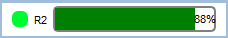
\includegraphics[width=0.4\textwidth]{Abbildungen/BatterieAlive2.png}
    \caption{Roboterstatus-LED blinkend}		
    \label{fig:Led}
\end{figure}

Über die Funktion UpdateRobotinoAlive() kann die LED aktiviert oder deaktiviert werden. Wenn der Roboter nicht mehr "`lebend"' ist wird eine Meldung an das Log geschrieben und die LED grau gesetzt (Abb. \ref{fig:Batterie} R5). 


Über den internen blink-Timer wird alle 500 ms die Funktion ToggleAliveRobotino() aufgerufen. In dieser Funktion wird für alle Robotinos, die "`lebend"' sind, die LED zwischen hellgrün und dunkelgrün gewechselt. Dies geschieht über eine Anpassung des Stylesheets von der LED (siehe Listing \ref{lst:LEDtoggle}). 

\begin{lstlisting}[frame=single, breaklines=true, numbers=left, stepnumber=2, firstnumber=1, numberstyle = \tiny, caption=Stylesheet Aktualisierung der Alive-LED ,label=lst:LEDtoggle]
toggler ? AliveR1->setStyleSheet("QPushButton {background-color: rgb(0,250,50); border-radius: 6px;}") : AliveR1->setStyleSheet("QPushButton {background-color: green; border-radius: 6px;}");
\end{lstlisting}

\section{Prozesseingabe}
\label{sec:Prozesseingabe}

Über den Bereich der Prozesseingabe (V) kann der Fertigungsplanung ein neuer Referenzprozess hinzugefügt werden (siehe Abb. \ref{fig:Prozesseingabe}). Durch die Markierung auf der linken Seite können die Prozessschritte ausgewählt werden, die dem Prozess hinzugefügt werden sollen. Über das UI können Prozesse mit 1 bis 5 Prozessschritten erzeugt werden. Nach Auswahl des Prozessschritts kann eine Station zwischen 2 und 7 ausgewählt werden. Sollten zwei aufeinanderfolgende Prozessschritte die selbe Station beinhalten, wird ein Fehler generiert. Zuletzt kann im rechten Eingabefenster die Bearbeitungsdauer an der Station zwischen 1 und 99 Sekunden ausgewählt werden.

\begin{figure}[htb]
    \centering
    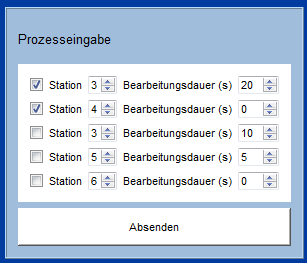
\includegraphics[width=0.5\textwidth]{Abbildungen/Prozesseingabe.png}
    \caption{Visualisierung - Prozesseingabe}		
    \label{fig:Prozesseingabe}
\end{figure}

Bei Anklicken des Buttons "`Absenden"' wird die Funktion on\_sendProzess\_clicked() aufgerufen. In der Funktion werden die Visualisierungseinträge von oben nach unten überprüft und die Prozessschritte zu einem Prozess erzeugt. Der letzte Prozessschritt zu Station 8 wird automatisch ergänzt. Abschließend wird der neue Prozess an die Fertigungsplanung und darüber an die Datenbank gesendet. 

\section{Auftragseingabe}
\label{sec:Auftragseingabe}

In Abbildung \ref{fig:Auftragsvergabe} ist Bereich VI abgebildet, in dem neue Aufträge erzeugt und dem Programm hinzugefügt werden können. 

\begin{figure}[htb]
    \centering
    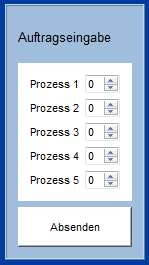
\includegraphics[width=0.25\textwidth]{Abbildungen/Auftragsvergabe.png}
    \caption{Visualisierung - Auftragsvergabe}		
    \label{fig:Auftragsvergabe}
\end{figure}

Um einen Auftrag zu erzeugen muss die Anzahl der zu bearbeitenden Referenzprozesse angegeben werden. Über die Tooltips (vgl. Abschnitt {sec:tooltips}) kann erkannt werden, was für Prozessschritte in den einzelnen Prozessen abgebildet sind. 

Bei Betätigung des Buttons "`Absenden"' werden die Felder zurückgesetzt und ein neuer Auftrag wird in der Fertigungsplanung erzeugt. 

In der Funktion AddAuftragsItem() werden anschließend die UI-Elemente in der Auftragsübersicht erzeugt. Der in Listing \ref{lst:AddAuftragsItem} dargestellte Code enthält die wesentlichen Codezeilen der Funktion. 

\begin{lstlisting}[frame=single, breaklines=true, numbers=left, stepnumber=2, firstnumber=1, numberstyle = \tiny, caption=Funktionsinhalt AddAuftragsItem ,label=lst:AddAuftragsItem]
QListWidgetItem *listWidgetItem = new QListWidgetItem(AuftragListWidget);
AuftragListWidget->addItem(listWidgetItem);
Auftragsitem *auftragsItem = new Auftragsitem(a);
auftragsItem->SetLabelText("Auftrag " + QString::number(a->id));
auftragsItem->UpdateAuftragsFortschritt();
listWidgetItem->setSizeHint (auftragsItem->sizeHint());
AuftragListWidget->setItemWidget(listWidgetItem, auftragsItem);
listWidgetItem->setWhatsThis(WhatsThis[0]);

int itemrow = AuftragListWidget->row(listWidgetItem);
foreach (Prozess *p, a->Prozesse)
{
    Prozessitem *prozessItem = new Prozessitem(p);
    prozessItem->SetLabelText("Prozess " + QString::number(p->referenzId));
    prozessItem->UpdateProzessFortschritt();

    QListWidgetItem *widgetItem = new QListWidgetItem();

    AuftragListWidget->insertItem(itemrow+1, widgetItem);

    AuftragListWidget->setItemWidget(widgetItem, prozessItem);
    widgetItem->setSizeHint(prozessItem->sizeHint());
    widgetItem->setHidden(true);
    widgetItem->setWhatsThis(WhatsThis[1]);
    QString temp = "Werkstueck: " + QString::number(p->lfdId);
    prozessItem->setToolTip(temp);
    itemrow++;
}
\end{lstlisting}

In Zeile 1 wird ein neues ListWidgetItem erzeugt, welches als Elternwidget das AuftragsListWidget gesetzt bekommt. Dieses Item wird nun dem Elternwidget AuftragsListWidget hinzugefügt. In den Zeilen 3 bis 5 wird ein neues Objekt vom Auftragsitem erzeugt, welches dem AuftragsListWidget hinzugefügt wird. Dabei ist wichtig, die Größe des Items explizit zu setzen, da es sonst eine Höhe von 1 Pixel bekommt. In Zeile 7 wird zuletzt das Auftragsitem der Liste angehängt. Das Item bekommt eine eindeutige Kennung, anhand derer ausgewertet wird, dass es sich um ein Auftragsitem handelt.

Nachdem das Auftragsitem erzeugt wurde, werden alle zugehörigen Prozessitems erzeugt. Das Vorgehen ähnelt den Zeilen 1 - 7, nur werden die Prozessitems dem zuvor erzeugtem AuftragsListWidget an einer bestimmten Stelle eingefügt (Zeile 19). Bei der Erzeugung werden die Prozessitems direkt ausgeblendet (Zeile 23). Zuletzt wird der Tooltip (siehe Abschnitt \ref{sec:tooltips}) für die Prozessitems in Zeile 26 generiert.

Das besondere an dieser Funktion ist, dass dynamisch zur Laufzeit Widget-Elemente erzeugt, und in die in die Visualisierung eingebunden werden. 

\section{Tooltips}
\label{sec:tooltips}

Um die Benutzerinteraktion zu erleichtern, wurden an zwei Stellen innerhalb der Visualisierung Tooltips implementiert. Ein Tooltip ist ein Hinweistext zu einem Element, der sich beim überfahren mit der Maus (hovern) neben dieser öffnet. 

\subsection{Werkstückstooltip}

Sobald die Maus über ein Arbeitsplatz gefahren wird, auf dem ein Werkstück liegt, oder eine Reservierung für ein Werkstück existiert, wird über den Tooltip angezeigt, welche ID dieses Werkstück besitzt. In Abbildung \ref{fig:Stationstooltip} ist dies anhand einer Reservierung für Werkstück 7 angezeigt. 

\begin{figure}[htb]
    \centering
    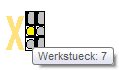
\includegraphics[width=0.31\textwidth]{Abbildungen/Werkstueckhover.png}
    \caption{Tooltip eines Werkstücks}		
    \label{fig:Stationstooltip}
\end{figure}

Die Tooltips eines Arbeitsplatzes werden über die Funktion UpdateStationToolTip() aktualisiert und über die Fertigungsplanung aufgerufen. 

\subsection{Prozessitemtooltip}

In Abbildung \ref{fig:Prozessitemtooltip} ist exemplarisch der Tooltip für Prozess 4 dargestellt. Dieser wird angezeigt, sobald mit der Maus über den Text des Prozesses gefahren wird. 

Der Im Tooltip dargestellte Text wird über die Funktion UpdateProzessLabelTooltip() verändert und aktualisiert. Dazu wird jeder Prozessschritt des Prozesses durchgegangen und ein String generiert, der die Station und die Bearbeitungsdauer enthält. Die einzelnen Strings werden untereinander dargestellt. 

\begin{figure}[htb]
    \centering
    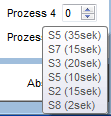
\includegraphics[width=0.25\textwidth]{Abbildungen/Prozesshover.png}
    \caption{Tooltip eines Prozessitem}		
    \label{fig:Prozessitemtooltip}
\end{figure}
